\documentclass{article}
\usepackage{graphicx} % Required for inserting images
\usepackage{fancyhdr} % Required for header and footer configuration
\usepackage[a4paper, margin=2.5cm, left=1.5cm, right=1.5cm, bottom=4cm]{geometry} % Required for setting page margins
\usepackage[T1]{fontenc}
\usepackage[default,oldstyle,scale=1]{opensans} % Utilizzo del font Open Sans
\usepackage{lipsum} 
\usepackage{makeidx}
\usepackage{booktabs}
\usepackage{tabularray}
\usepackage[colorlinks=true, linkcolor=black, urlcolor=blue, citecolor=blue]{hyperref}
\usepackage{tabularx}
\usepackage{makecell}

% Configure header and footer for the first page
\fancypagestyle{firstpage}{
    \fancyhf{} % Clear header and footer
    \renewcommand{\headrulewidth}{0pt} % Remove header rule line
    \lhead{} % Header on the left
    \chead{} % Header in the center
    \rhead{} % Header on the right
    \lfoot{} % Footer on the left
    \cfoot{\vspace{5pt}\\\hrulefill\\\vspace{10pt}\textbf{BeeLive}\\Gruppo 21} % Footer in the center
    \rfoot{\vspace{32.5pt}\\\thepage} % Footer on the right
}

% Configure header and footer for non-plain pages (second page onwards)
\fancypagestyle{nonplain}{
    \fancyhf{} % Clear header and footer
    \lhead{} % Header on the left
    \chead{} % Header in the center
    \rhead{
\includegraphics[width=2cm]{Images/BeeLive-Logo.png}\\\vspace{2pt}} % Header on the right
    \lfoot{} % Footer on the left
    \cfoot{\vspace{5pt}\\\hrulefill\\\vspace{10pt}\textbf{BeeLive}\\Gruppo 21} % Footer in the center
    \rfoot{\vspace{32.5pt}\\\thepage} % Footer on the right
}

% Adjust vertical space between header and text
\setlength{\headsep}{65pt} 
% Adjust vertical space between text and footer
\setlength{\footskip}{0pt} 

\title{
\includegraphics[width=0.75\textwidth]{Images/BeeLive-Logo.png}\\\vspace{100pt}
\LARGE{\textbf{BeeLive\\Deliverable 1}}}
\author{Gruppo 21:\\
Cipriani Pietro, 226959\\
Orlando Dennis, 227688\\
Ziviani Elia, 228172}
\date{28 Marzo 2024}

\makeindex % Indica che vogliamo creare un indice

\begin{document}

\maketitle
\thispagestyle{firstpage} % Apply firstpage style to the first page
\clearpage

\pagestyle{nonplain} % Apply non-plain style to subsequent pages

\renewcommand{\contentsname}{Indice}
\tableofcontents

\clearpage
\section{Descrizione dell'applicativo}
\index{Descrizione dell'applicativo} % Aggiunge una voce all'indice
La Municipalità di Trento ha richiesto la valutazione dei problemi cittadini e la proposta di soluzioni attraverso lo sviluppo di un'applicazione web ad-hoc.

Dopo un processo di ideazione, è emerso che a Trento risulta spesso difficile reperire informazioni riguardanti gli eventi che influenzano la viabilità stradale. Le informazioni disponibili sono principalmente testuali e richiedono un impegno attivo da parte dei cittadini per essere trovate, poiché attualmente manca un sistema di notifica automatica per tali modifiche.

Di conseguenza, l'idea concepita prevede lo sviluppo di un sistema informativo che consenta ai cittadini di accedere rapidamente ed intuitivamente a tutte le variazioni della viabilità, senza la necessità di una ricerca attiva.\\

Il nucleo concettuale si basa sulla rappresentazione grafica delle zone coinvolte nelle modifiche della viabilità, per facilitare la comprensione delle informazioni.\\
È inoltre previsto un sistema di notifiche push per informare i cittadini in tempo reale sugli eventi che coinvolgono l'intera città o solo le zone da loro selezionate.\\

Saranno sviluppati due ambienti distinti: Uno riservato all'amministrazione e uno accessibile ai cittadini.\\
Il primo ambiente consentirà all'amministrazione di inserire e modificare le informazioni sulle variazioni della viabilità attraverso un'interfaccia grafica intuitiva e compatibile con gli standard per la visualizzazione dei dati su mappa.\\
Il secondo sarà un'applicazione mobile installabile sui dispositivi dei cittadini, che consentirà loro di visualizzare graficamente le zone interessate dai cambiamenti, selezionare le aree di loro interesse e ricevere notifiche push in tempo reale.

Ogni variazione inserita nel sistema dall'amministrazione sarà caratterizzata dalla zona interessata, visualizzabile sulla mappa, da una descrizione che ne spiega la natura e da una stima della durata della variazione, tutte informazioni che i cittadini potranno visualizzare tramite l'applicazione mobile dal loro dispositivo.
\clearpage

\clearpage

\section{Obiettivi}
\index{Obiettivi} % Aggiunge una voce all'indice

Cosa dovrebbe fare l'applicativo, descrizione punto per punto.\\

\clearpage

\section{Attori di sistema e Mind map}
\index{Attori di sistema e Mind map} % Aggiunge una voce all'indice

\subsection{Attori di sistema}
\index{Attori di sistema}

Va definito chi fa cosa nel sistema, tutte le entità che hanno a che fare con il sistema
\begin{itemize}
    \item Who will use the functionality of the system?
    \item Who will maintain the system?
    \item What devices does the system need to handle?
    \item What other system does this system need to interact?
    \item Who or what has interest in the results of this system?
\end{itemize}

\clearpage

\subsection{Mind map}
\index{Mind map}

%\begin{figure}[htbp]
%    \label{fig:Mind_map}
%    \centering
%    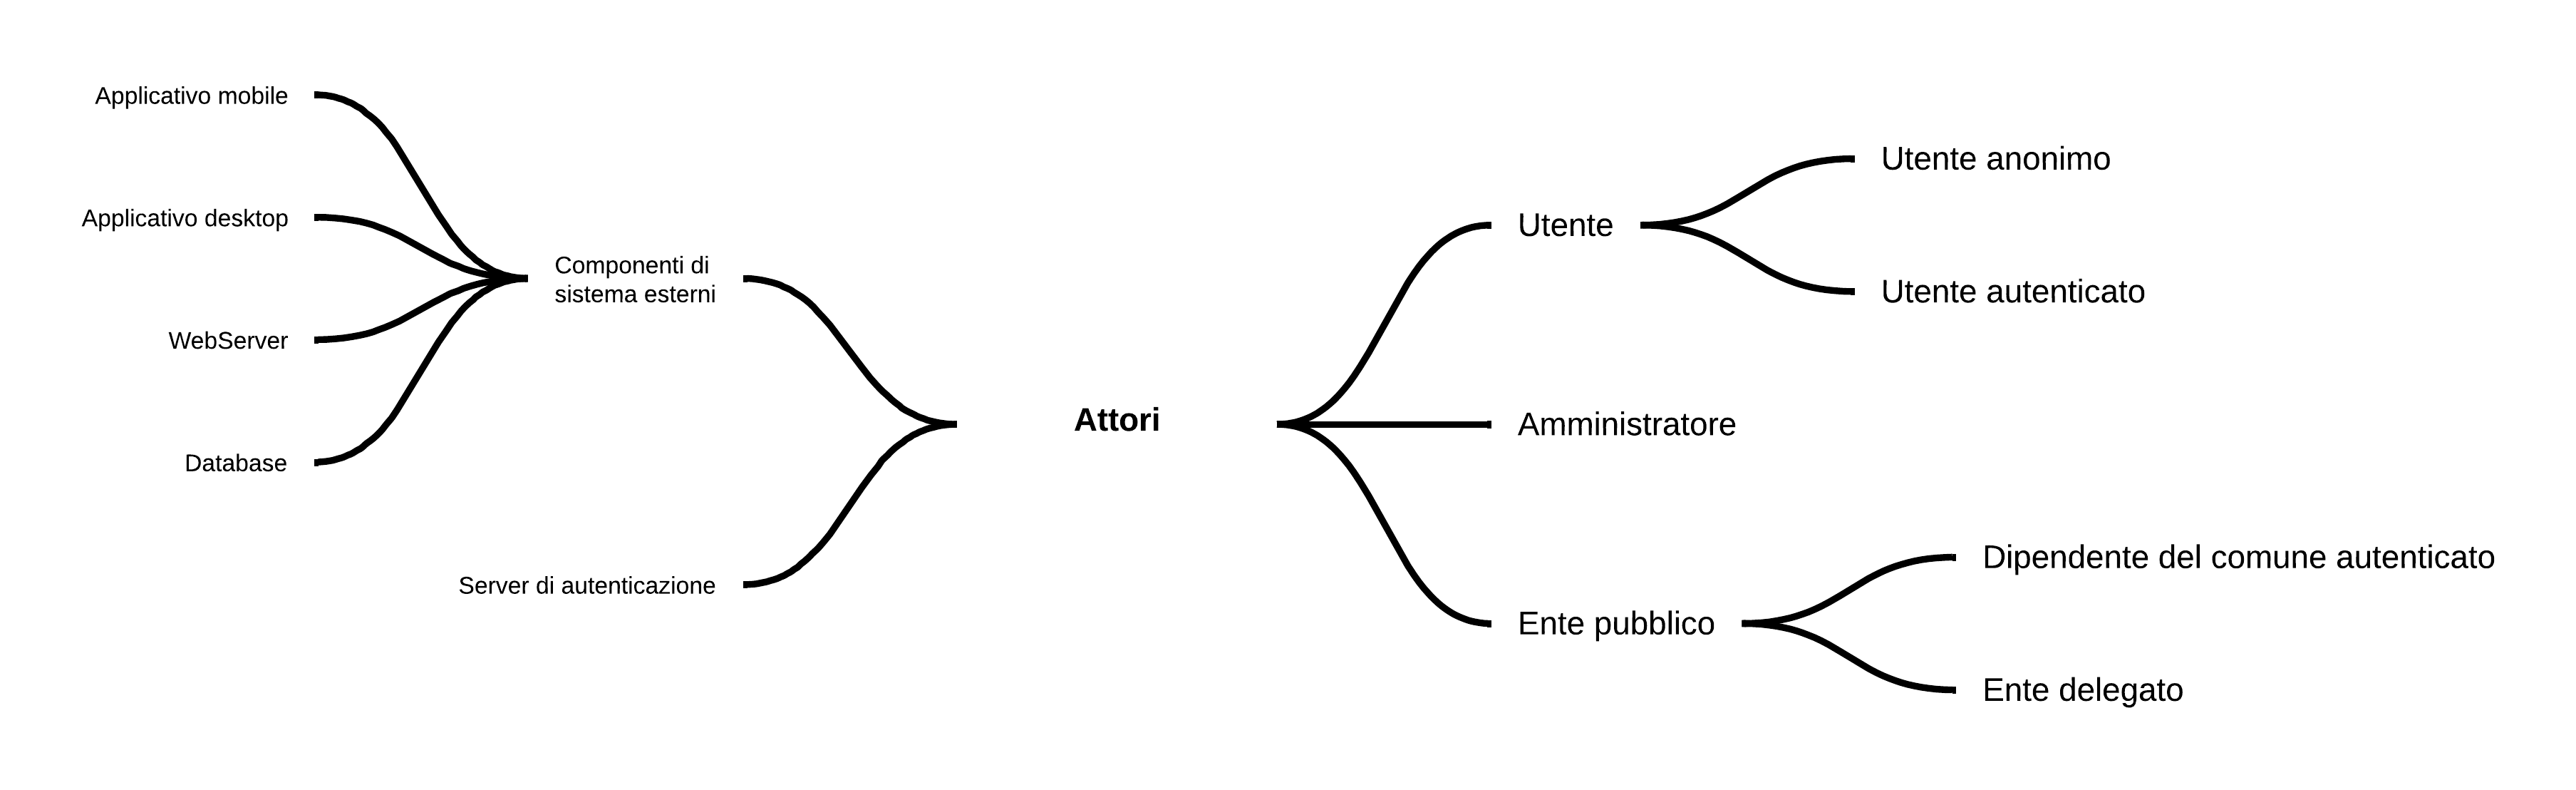
\includegraphics[width=0.5\textwidth]{Images/MindMap.png}
%    \caption{Mind map degli attori che interagiscono con il sistema}
%\end{figure}

Tramite la mind map è possibile avere una rappresentazione chiara degli attori che interagistocno con il sistema.\\
\clearpage

\section{Prototipo}
\index{Prototipo} % Aggiunge una voce all'indice

\subsection{Mockup applicazione mobile}
\index{Mockup applicazione mobile} % Aggiunge una voce all'indice\usepackage{makecell}

\subsubsection{Schermata principale}
\index{Schermata principale} % Aggiunge una voce all'indice
\begin{figure}[htbp]
    \label{fig:Schermata_principale_mobile}
    \centering
    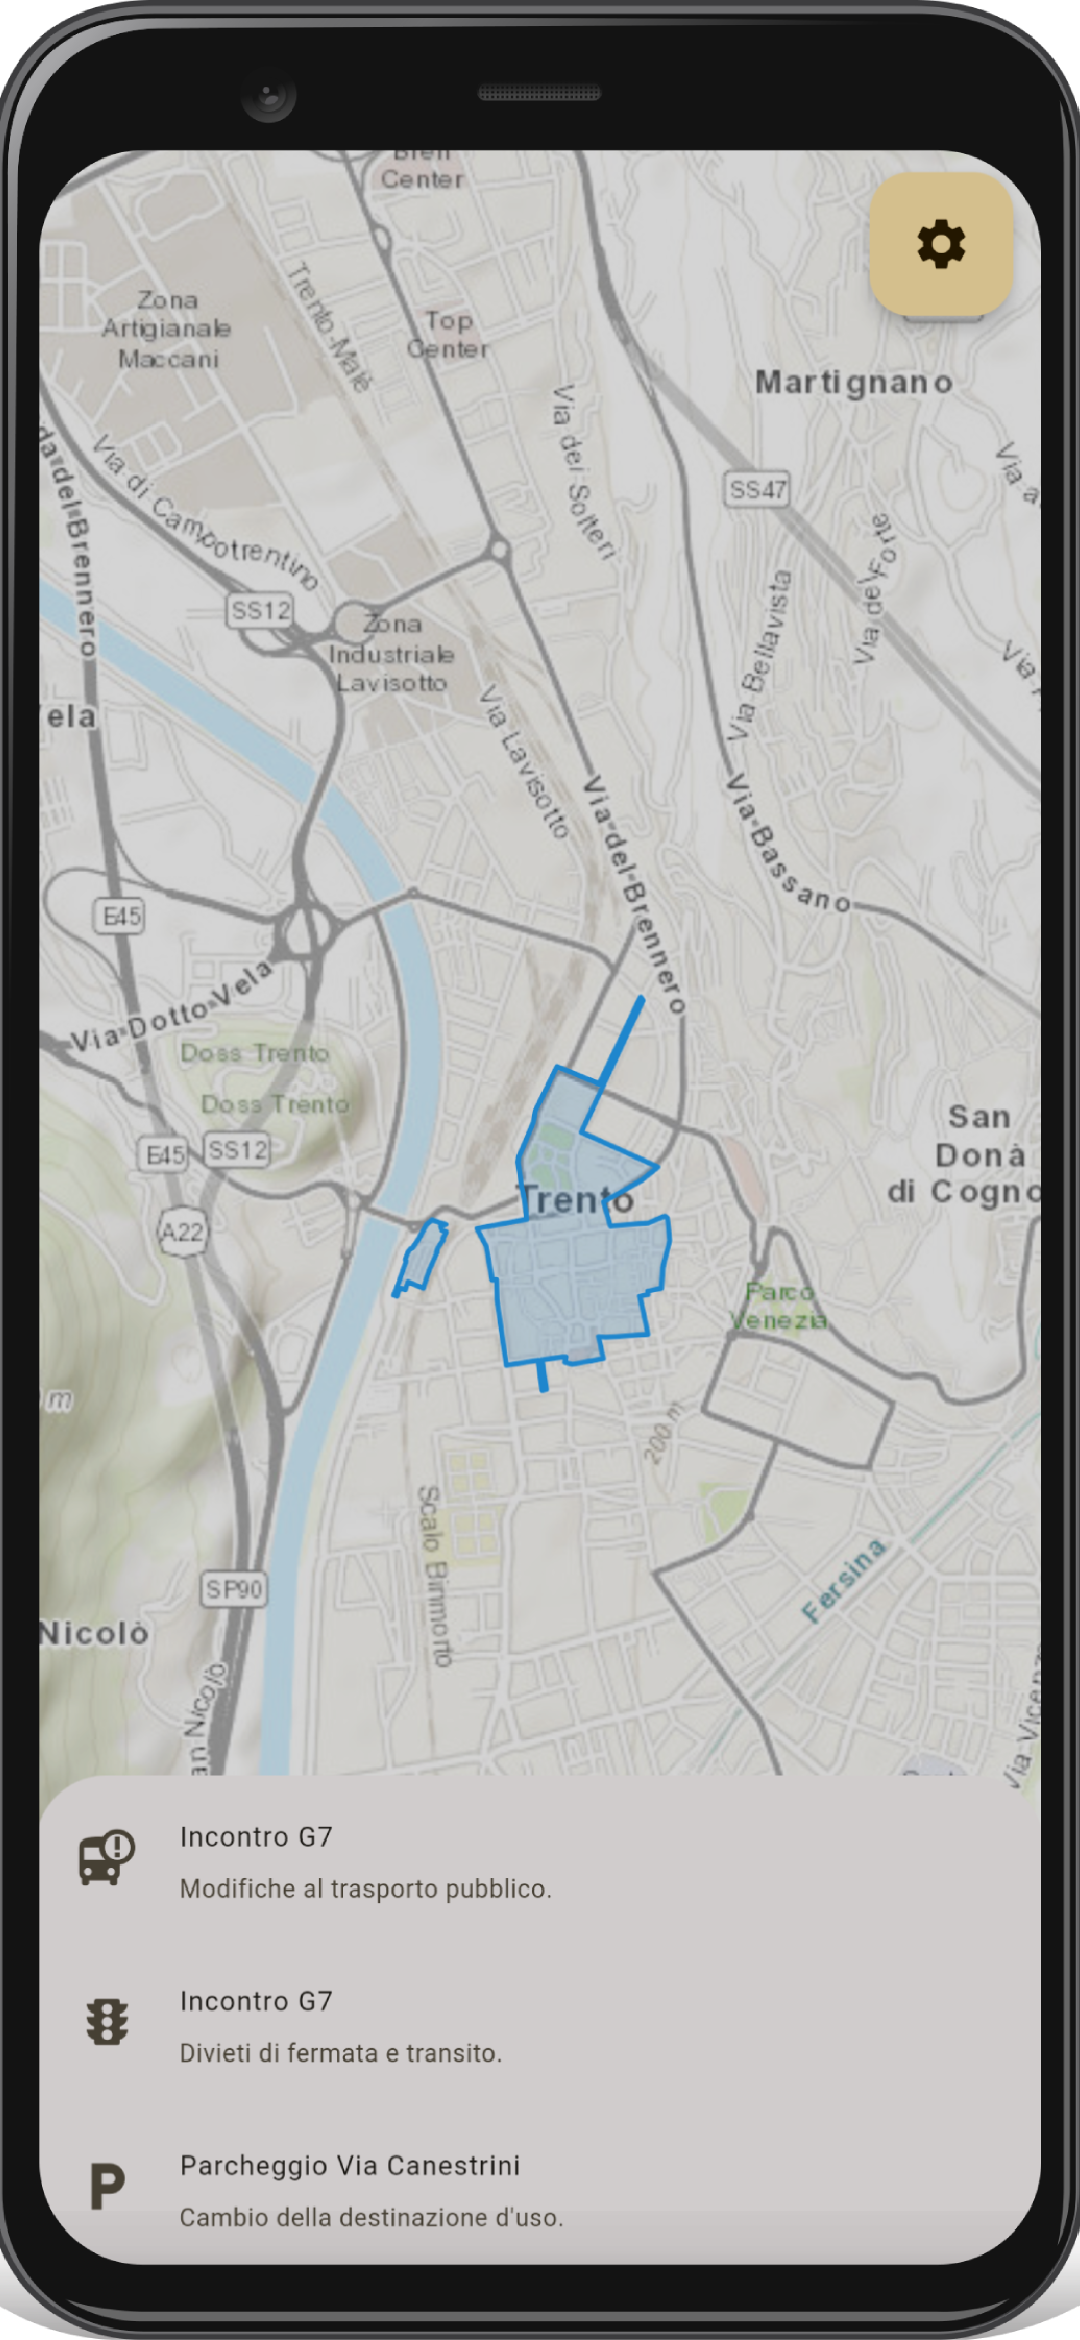
\includegraphics[width=0.25\textwidth]{Images/Mockup1 - Mobile.png}
    \caption{Mockup schermata principale dell'applicazione mobile}
\end{figure}

E' rappresentata la schermata principale dell'applicazione mobile che il cittadino installerà sul proprio smartphone.\\
La schermata principale mostra una mappa della città di Trento con le zone interessate dalle variazioni della viabilità.\\
La lista sottostante la mappa riporta tutte le variazioni presenti nel sistema che si trovano nel periodo di visualizzazione, con la possibilità di selezionare una variazione per visualizzarne i dettagli.\\
\clearpage

\subsubsection{Dettagli variazione selezionata}
\index{Dettagli variazione selezionata} % Aggiunge una voce all'indice
\begin{figure}[htbp]
    \label{fig:Dettaglio_evento}
    \centering
    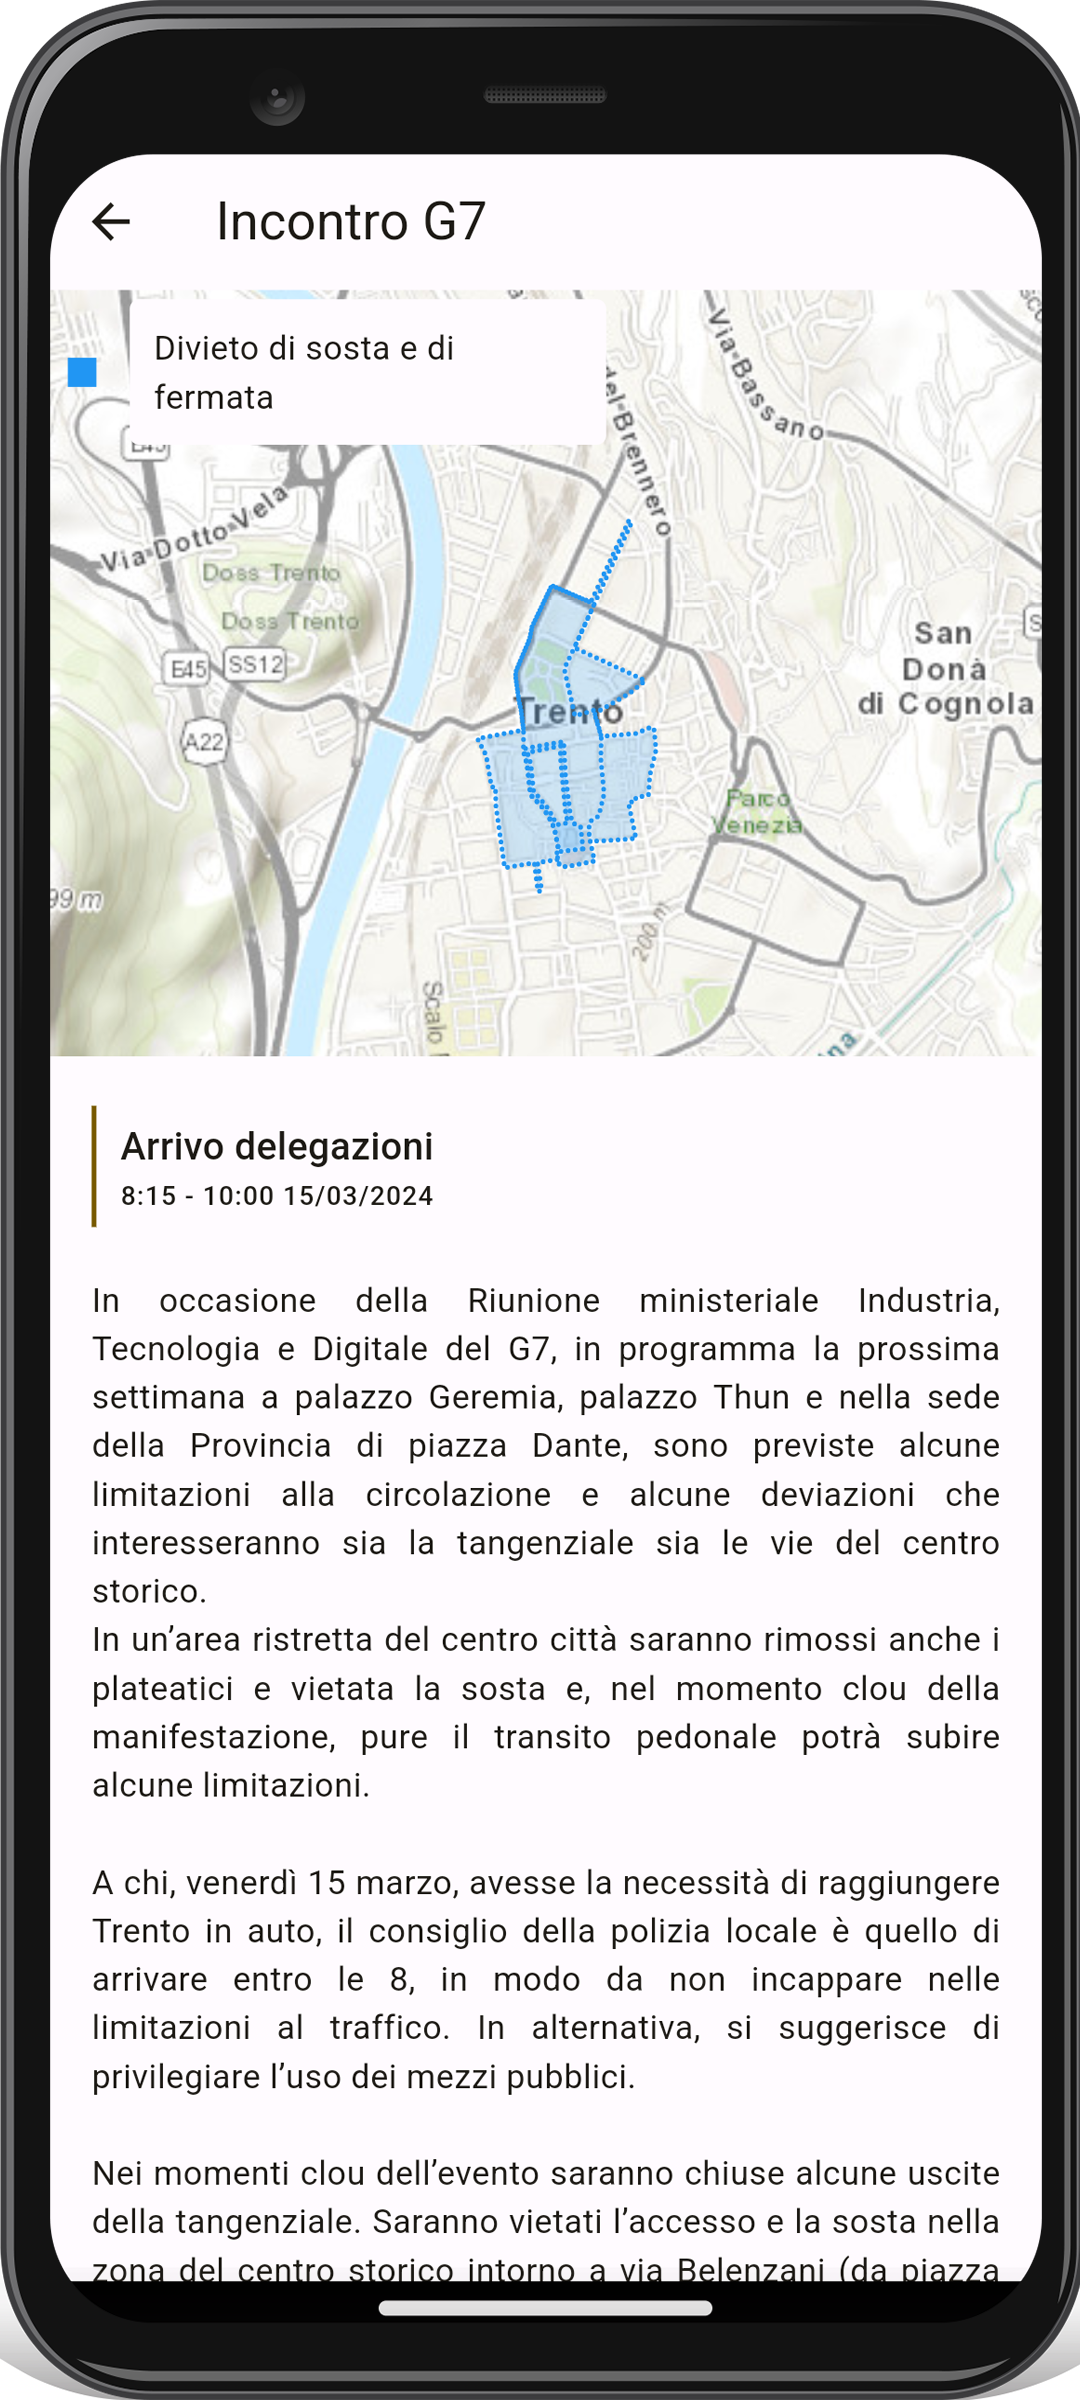
\includegraphics[width=0.25\textwidth]{Images/Mockup2 - Mobile.png}
    \caption{Mockup schermata detagli di un evento dell'applicazione mobile}
\end{figure}

In questo caso invece è riportata la schermata di visualizzazione dei dettagli di una variazione della viabilità.\\
E' stato selezionato il precedente evento "Incontro G7", quindi sono visualizzati tutti i dettagli relativi a tale evento.\\
Nella fattispecie sono presenti la descrizione dell'evento, la data di inizio e fine, la zona interessata e la mappa con la visualizzazione della zona interessata.\\
Inoltre è presente un pulsante per tornare alla schermata principale dell'applicazione.\\
\clearpage

\subsubsection{Mockup notifiche degli eventi}
\index{Mockup notifiche degli eventi} % Aggiunge una voce all'indice

\begin{figure}[htbp]
    \label{fig:Notifica_evento}
    \centering
    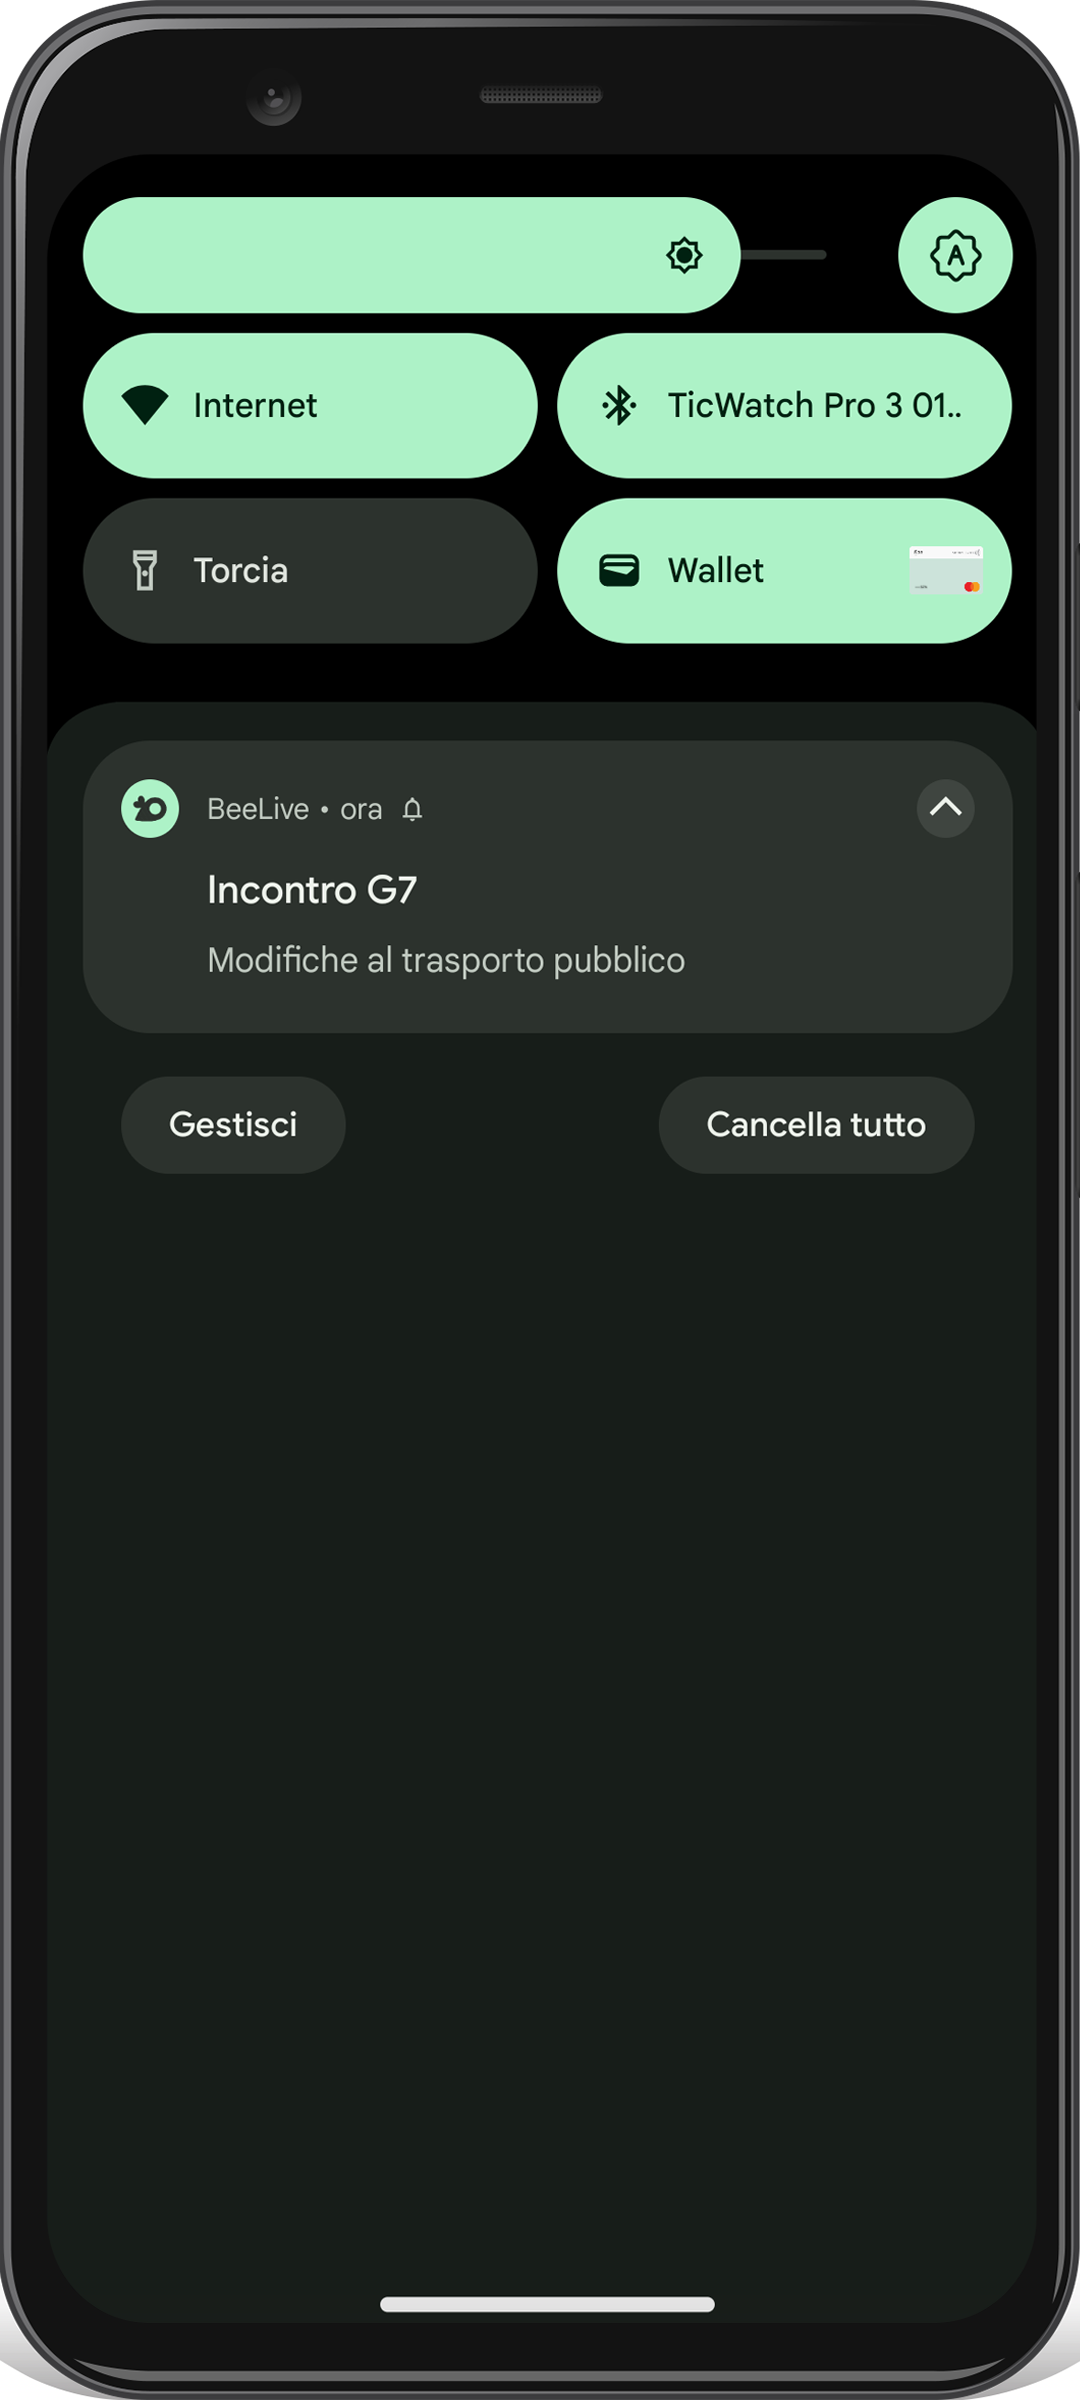
\includegraphics[width=0.25\textwidth]{Images/Mockup3 - Mobile.png}
    \caption{Mockup notifiche generate da un'evento dall'applicazione mobile}
\end{figure}

L'evento preso nell'esempio precedente era impostato per generare delle notifiche push.\\
Quella riportata nell'esempio soprastante rappresenta la notifica di inizio dell'evento "Incontro G7".\\
Interagendo con essa sarà quindi aperta l'applicazione mobile sulla schermata riportata in \hyperref[fig:Dettaglio_evento]{figura 2}, permettendo quindi la consultazione delle modifiche per intero.\\

\clearpage

\subsection{Mockup interfaccia desktop}
\index{Mockup interfaccia desktop} % Aggiunge una voce all'indice
%Immagine singola
\begin{figure}[htbp]
    \label{fig:Schermata_principale_desktop}
    \centering
    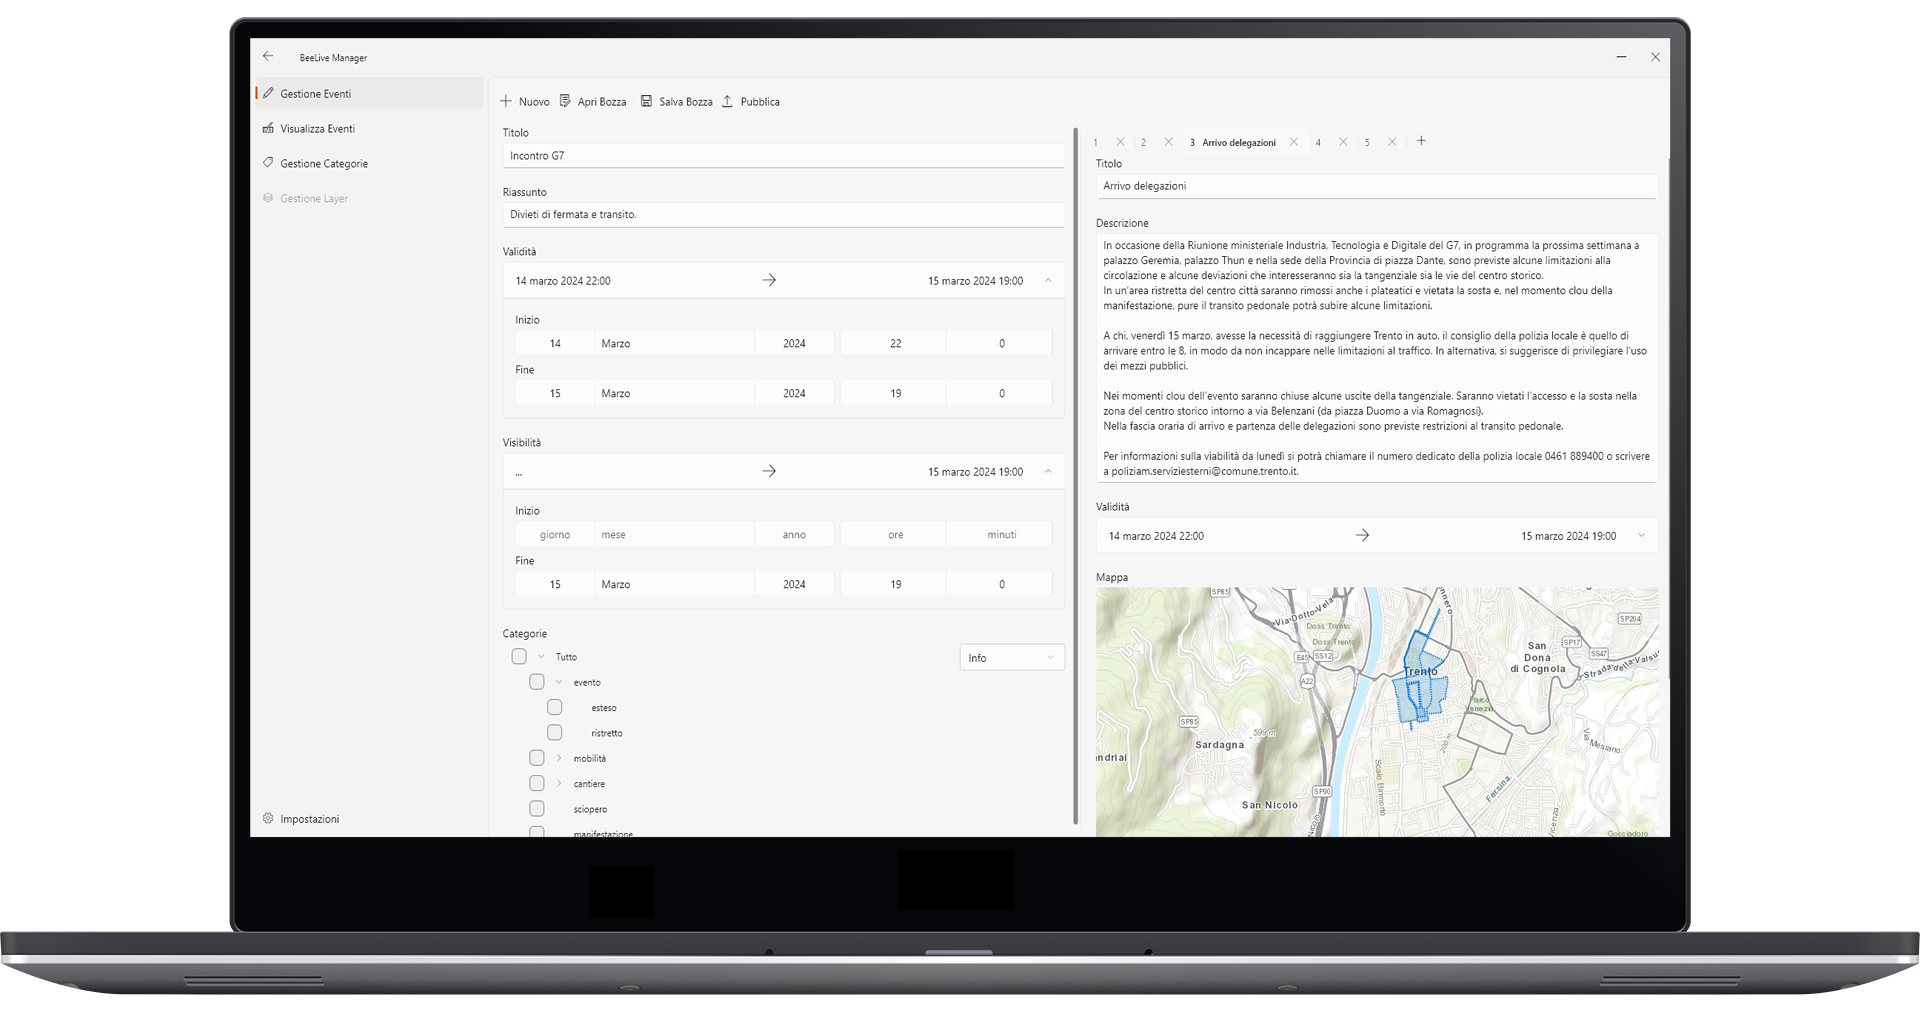
\includegraphics[width=0.75\textwidth]{Images/Mockup1 - Desktop.png}
    \caption{Mockup dell'interfaccia amministrativa}
\end{figure}

L'immagine rappresenta come dovrebbe essere strutturata l'interfaccia dell'applicativo desktop, utilizzato dagli enti pubblici con potere di amministrazione per la pobblicazione degli eventi in città che ne influenzano la viabilità.\\
L'interfaccia comprende un menu laterale per la navigazione tra le varie sezioni dell'applicativo e la schermata dove il sottomen selezionato presenta tutte le sue specifiche funzionalità disponibili.

Il sottomenù selezionato in questo caso è "Gestione Eventi", la sezione in cui è possibile inserire un nuovo evento che modifica la viabilità cittadina. Infatti sono riportati tutti i campi necessari per la creazione di un evento, come il titolo, il riassunto, la data di inizio e fine di validità dell'evento e di visibilità sull'applicativo mobile, e le categorie che caratterizzano l'evento.

L'interfaccia è strutturata in modo che ogni evento abbia la possibilità di essere composto da più sottoeventi. Nella sezione di destra è possibile visualizzare l'inderimento del sottoevento "Arrivo delle delegazioni", dove è possibile inserire il titolo, la descrizione, la data di validità e la zona interessata direttamente su mappa.\\

\clearpage

\section{Requirements}
\index{Requirements}
\begin{enumerate}
    \item Condition or capability needed by a user to solve a problem or achieve an objective
    \item A condition or capability that must be met or possessed by a system or component to satisfy a contract, standard, specification, or other
    \item A documented representation of a condition or capability as in (1) or (2)
\end{enumerate}

\subsection{Requirements funzionali}
\index{Requirements funzionali} % Aggiunge una voce all'indice

Per ogni attore, mostrare quello che può fare

\clearpage

\subsection{Requirements non funzionali}
\index{Requirements non funzionali} % Aggiunge una voce all'indice

\subsubsection{Affidabilità delle informazioni pubblicate}
\index{Affidabilità delle informazioni pubblicate}

E' necessario che le informazioni che i cittadini andranno a consultare siano affidabili e provenienti da fonti verificate.\\

\subsubsection{Portabilità}
\index{Portabilità}

Il sistema, come descritto in precedenza, è composto da due moduli: L'applicazione mobile e il programma desktop.
L'applicazione mobile deve poter essere installata e funzionare in modo responsivo sugli smartphone Apple, che devono essere dotati di almento una versione del sistema IOS superiore alla 13, mentre per tutti gli altri deve essere installata una versione di Android uguale o successiva alla 8.0.1
L'applicativo desktop invece (Decisione se WebApp oppure nativo)

\subsubsection{Responsività applicazione mobile}
\index{Responsività applicazione mobile}
\begin{itemize}
    \item Il popolamento della lista degli eventi di modifica della viabilità deve essere eseguito in un tempo non superiore ai 5 secondi.
    \item Il tempo che trascorre per l'ottenimento delle informazioni dell'evento selezionato che devono essere mostrate al cittadino non deve essere superiore ai 5 secondo.
    \item Le notifiche devono apparire sul dispositivo sul quale è installata l'applicazione mobile in un tempo minore o uguale a 5 secondi.
\end{itemize}

\subsubsection{Responsività programma desktop}
\index{Responsività programma desktop}
Decidere come realizzare l'applicazione per completare
\begin{itemize}
    \item Il tempo di pubblicazione di un evento, una volta compilati tutti i campi ed inviata la richiesta, non deve essere superiore a 5 secondi.
    \item Se richiesto all'applicativo di gestire un file d'informazione spaziale (GeoJson o simili), non deve intercorrere un tempo superiore ad 1 minuto.
\end{itemize}

\subsubsection{Usabilità}
\index{Usabilità}
\label{useCase:Usabilità}

Il semplice cittadino, una volta installata l'applicazione, deve poter consultare tutti i dati relativi alle modifiche di viabilità senza nessun tipo di addestramento. Nel caso in cui effettui il login, deve essere in grado di eseguire tutte le funzioni dell'utente riconosciuto in autonomia.\\
L'ente pubblico che decide di pubblicare una modifica di viabilità deve poterlo fare in modo semplice e veloce, a seguito di un breve corso di formazione di al massimo 10 minuti.\\
L'ente che invece si occupa di validare le variazioni di viabilità deve poterlo fare in modo comodo e autonomo, dopo aver seguito un corso di formazione di al massimo 10 minuti.\\

Integrare con altre funzioni necessarie

\subsubsection{Scalabilità}
\index{Scalabilità}

Integrare con funzionalità definite nei requirements funzionali

Il sistema deve essere in grado di mantenere le performace citate in precedenza al punto \hyperref[useCase:Usabilità]{Usabilità} anche in caso di:
\begin{itemize}
    \item Illimitati utenti che consultano simultaneamente l'applicazione mobile
    \item 100 enti pubblici che pubblicano eventi di modifica della viabilità in modo simultaneo
\end{itemize}
\clearpage

\section{Grafo BPMN}
\index{Grafo BPMN} % Aggiunge una voce all'indice
\clearpage

\section{Diagramma dei casi d'uso}
\index{Diagramma dei casi d'uso} % Aggiunge una voce all'indice

% Template tabella casi d'uso

\begin{table}[htbp]
\begin{tabular*}{\textwidth}{ @{\extracolsep{\fill}} || l | p{0.8\textwidth} || }
    \hline
    Nome caso d'uso & *Nome* \\
    \hline\hline
    ID & Testo \\
    \hline
    Descrizione & Testo \\
    \hline
    Attori primari & Testo \\
    \hline
    Attori secondari & Testo \\
    \hline
    Precondizioni & Testo \\
    \hline
    Flusso principale & Testo \\
    \hline
    Post-condizioni & Testo \\
    \hline
    Flussi alternativi & Testo \\
    \hline
\end{tabular*}
\end{table}

\clearpage

\section{Resoconto}
\index{Resoconto} % Aggiunge una voce all'indice

Segue la tabella dei riferimenti, utile alla comprensione generale delle diverse sezioni riguardanti lo specifico obiettivo.\\

\begin{table}[htbp]
    \centering
    \begin{tabularx}{\textwidth}{|X|X|X|X|X|X|}
        \Xhline{2pt} % Linea spessa
        Obiettivo & Attore & User Story & Use Case\newline diagram & Requisiti\newline funzionali & Mockup \\
        \Xhline{2pt} % Linea spessa
        1 & 2 & 3 & 4 & 5 & 6 \\
        \hline
    \end{tabularx}
    \caption{Tabella riassuntiva}
    \label{tab:tabella_tutta_pagina}
\end{table}

\end{document}
